\chapter{Масштабирование моделей}
\label{chap:deep_cnns}

\begin{supportbox}{Об этой главе}
Теперь мы переходим к задаче проектирования дифференцируемых моделей, имеющих десятки (или сотни) слоев. Как мы видели, рецептивное поле свёрточных моделей растет линейно с числом слоев, что мотивирует архитектуры с такой глубиной. Это можно сделать, правильно стабилизировав обучение с помощью множества методов, от аугментации данных до нормализации скрытых состояний.
\end{supportbox}


\section{Соревнование ImageNet}

Давайте снова рассмотрим задачу классификации изображений, которая представляет большой интерес для нейронных сетей, как с практической, так и с исторической точки зрения. Фактически, интерес к этим моделям в период 2012-2018 годов можно в значительной степени связать с \textbf{ImageNet Large Scale Visual Recognition Challenge}\footnote{\url{https://image-net.org/challenges/LSVRC/}} (далее для простоты \textbf{ImageNet}). ImageNet — это ежегодное соревнование, которое проводилось с 2010 по 2017 год для оценки самых современных моделей для классификации изображений. Соревнование проводилось на подмножестве всего набора данных ImageNet, состоящем примерно из 1 млн изображений, помеченных по 1 тыс. классов. 

Поучительно взглянуть на ранние выпуски соревнований. В 2010\footnote{\url{https://image-net.org/challenges/LSVRC/2010/}} и в 2011 годах\footnote{\url{https://image-net.org/challenges/LSVRC/2011/}} победителями были методы линейных ядер, построенные с использованием комбинации специализированных дескрипторов изображений и ядер, с ошибкой топ-5\% в 28\% (2010) и 26\% (2011). Несмотря на ряд многообещающих результатов,\footnote{\url{https://people.idsia.ch/~juergen/computer-vision-contests-won-by-gpu-cnns.html}} свёрточные модели, обученные градиентным спуском, оставались нишевой темой в компьютерном зрении. Затем, в 2012 году, модель-победитель (AlexNet, \cite{krizhevsky2012imagenet}) достигла ошибки топ-5\% в 15.3\%, что на 10\% ниже, чем у всех (не нейронных) конкурентов. 

За этим последовала настоящая «коперниканская революция» (прошу прощения у Коперника) в этой области, поскольку за несколько лет почти все заявки перешли на свёрточные модели, и общая точность росла с беспрецедентной скоростью, превысив 95\% (что привело к завершению соревнования в 2017 году), как показано на Рисунке \ref{fig:papers_with_code}. За 5 лет свёрточные модели, обученные градиентным спуском, стали ведущей парадигмой в компьютерном зрении, включая другие подполя, которые мы здесь не упоминаем, от обнаружения объектов до семантической сегментации и оценки глубины.

\begin{SCfigure}
    \centering
    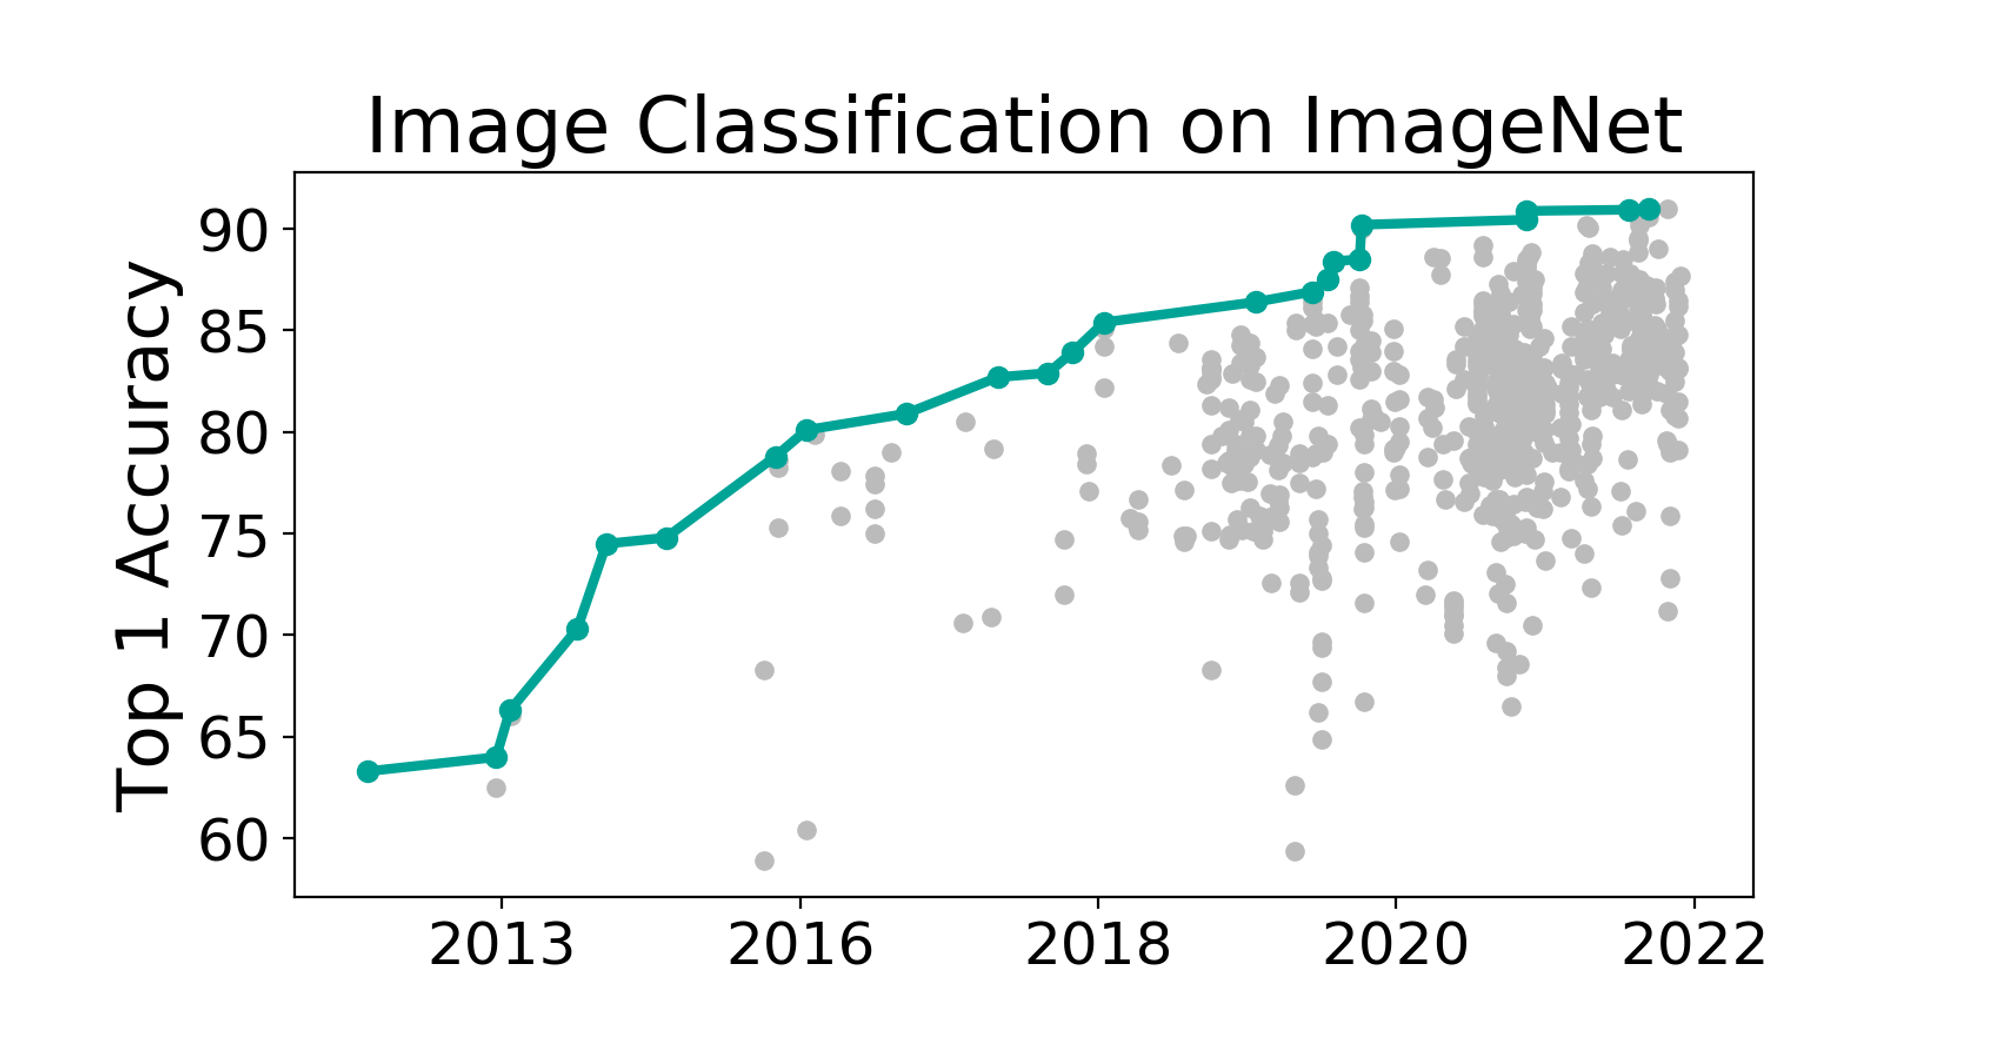
\includegraphics[width=0.6\textwidth]{images/imagenet}
    \caption[Воспроизведено из Papers With Code.]{Точность топ-1 на наборе данных ImageNet. Воспроизведено из Papers With Code.\footnote{\url{https://paperswithcode.com/}}}
    \label{fig:papers_with_code}
\end{SCfigure}

AlexNet была относительно простой моделью, состоящей из 5 свёрточных слоев и 3 полносвязных слоев, в общей сложности около 60 млн параметров, в то время как самые производительные модели на Рисунке \ref{fig:papers_with_code} требуют до сотен слоев. Это базовый пример закона масштабирования (Глава \ref{chap:introduction}): добавление слоев и вычислительной мощности для обучения пропорционально связано с точностью модели до точки насыщения, заданной набором данных. Однако масштабирование свёрточных моделей за пределы нескольких слоев нетривиально, поскольку оно сталкивается с рядом проблем, от медленной оптимизации до проблем с градиентами и численной нестабильности. Как следствие, в 2012-2017 годах был разработан большой набор техник для стабилизации обучения очень больших моделей.

В этой главе мы предоставляем обзор некоторых из этих техник. Мы сосредоточимся на идеях и методах, которые до сих пор являются фундаментальными, даже для других архитектур (например, трансформеров). Мы начнем с трех техник для улучшения обучения, которые хорошо известны в машинном обучении: \textbf{регуляризация весов}, \textbf{аугментация данных} и \textbf{ранняя остановка}. Затем мы опишем три из наиболее влиятельных техник, популяризированных в 2012-2017 годах: \textbf{dropout}, \textbf{пакетная нормализация} и \textbf{остаточные соединения}, более или менее в хронологическом порядке их введения. Для каждого метода мы опишем базовый алгоритм вместе с некоторыми вариантами, которые хорошо работают на практике (например, послойная нормализация).


\section{Данные и стратегии обучения}

\subsection{Регуляризация весов}

Один из возможных способов улучшить обучение — это наказывать решения, которые могут показаться неправдоподобными, например, имеющие один или два чрезвычайно больших веса. Обозначим через $\mathbf{w}$ вектор всех параметров нашей модели, а через $L(\mathbf{w}, \mathcal{S}_n)$ — функцию потерь на нашем наборе данных (например, среднюю кросс-энтропию). Мы можем формализовать предыдущую идею, определив так называемый \textbf{член регуляризации} $R(\mathbf{w})$, который оценивает решения на основе наших предпочтений, и наказывать потери, добавляя член регуляризации к исходной функции потерь:
\%
$$
L_{\text{reg}}=L(\mathbf{w}, \mathcal{S}_n)+\lambda R(\mathbf{w})
$$
\%
где мы предполагаем, что большее значение $R(\mathbf{w})$ соответствует худшему решению, а $\lambda \ge 0$ — это скаляр, который взвешивает два члена. При $\lambda=0$ член регуляризации не имеет эффекта, в то время как при $\lambda \rightarrow \infty$ мы просто выбираем лучшую функцию на основе наших априорных знаний.

Это также можно оправдать как выполнение вывода по максимуму апостериорной вероятности (вместо максимального правдоподобия) на основе комбинации априорного распределения по весам $p(\mathbf{w})$ и стандартной функции правдоподобия на наших данных (Раздел \ref{sec:bayesian_learning}):
\%
\begin{equation}
\mathbf{w}^*=\underset{\mathbf{w}}{\arg\max}\left\{ \log p(\mathcal{S}_n \;\vert\; \mathbf{w}) + \log p(\mathbf{w})\right\}
\label{eq:map_solution}
\end{equation}
\%
где наличие члена регуляризации соответствует неоднородному априорному распределению $p(\mathbf{w})$. Мы уже видели один пример регуляризации в Разделе \ref{subsec:regularizing_least_squares}, т.е. $\ell_2$-норму весов:
\%
$$
R(\mathbf{w})=\lVert \mathbf{w} \rVert^2 =\sum_i w_i^2
$$
\%
Для тех же нерегуляризованных потерь штрафование $\ell_2$-нормы будет благоприятствовать решениям с меньшей величиной весов, что соответствует «менее резким» изменениям на выходе при небольшом отклонении на входе.\footnote{По отношению к \eqref{eq:map_solution}, $\ell_2$-регуляризация эквивалентна выбору гауссовского априорного распределения по весам с диагональной ковариацией $\sigma^2 \mathbf{I}$.} Рассмотрим теперь влияние члена регуляризации на член градиента:
\%
$$
\nabla L_{\text{reg}}=\nabla L(\mathbf{w},\mathcal{S}_n)+2\lambda\mathbf{w}
$$
\%
Записанное в этой форме, это иногда называется \textbf{затуханием весов}, потому что в отсутствие первого члена его чистый эффект заключается в затухании весов на небольшой пропорциональный коэффициент $\lambda$ (отправляя их к $0$ экспоненциально быстро с числом итераций, если $\nabla L(\mathbf{w}, \mathcal{S}_n)=0$). Для (S)GD $\ell_2$-регуляризация и затухание весов совпадают. Однако для других типов алгоритмов оптимизации (например, SGD на основе момента, Adam) обычно применяется постобработка градиентов. Обозначая через $g(\nabla L(\mathbf{w}, \mathcal{S}_n))$ постобработанные градиенты (нерегуляризованных) потерь, мы можем записать обобщенную формулировку затухания весов (игнорируя постоянный член $2$) как:

$$
\mathbf{w}_t =\mathbf{w}_{t-1} \eqnmarkbox[drawred]{node}{-g(\nabla L(\mathbf{w}_{t-1}, \mathcal{S}_n))} \eqnmarkbox[drawgreen]{node2}{- \lambda \mathbf{w}_{t-1}}
$$
\annotate[yshift=1em]{above,right}{node}{Нерегуляризованный градиент}
\annotate[yshift=-1em]{below,right}{node2}{Член затухания весов}

Это отличается от чистой $\ell_2$-регуляризации, и в этом случае градиенты члена регуляризации находились бы внутри $g(\cdot)$. Это особенно важно для алгоритмов, таких как Adam, для которых формулировка затухания весов может работать лучше \cite{loshchilov2018fixing}.

Мы также можем рассмотреть другие типы членов регуляризации. Например, $\ell_1$-норма:
\%
$$
R(\mathbf{w})=\lVert \mathbf{w} \rVert_1=\sum_i \lvert x_i \rvert
$$
\%
может способствовать \textit{разреженным} решениям с высоким процентом нулевых значений (и это соответствует размещению априорного распределения Лапласа на весах). Это также можно обобщить на групповые разреженные варианты для обеспечения структурированной разреженности нейронов \cite{scardapane2017group}.\footnote{Обучение разреженных моделей — это огромная тема со многими связями также с эффективным выполнением на оборудовании. См. \cite{bach2012optimization} для обзора разреженных штрафов в контексте выпуклых моделей и \cite{hoefler2021sparsity} для обзора разреженности и обрезки в общих дифференцируемых моделях.}  Разреженное $\ell_1$-штрафование менее распространено, чем для других моделей машинного обучения, потому что оно плохо взаимодействует с сильной невыпуклостью задачи оптимизации и использованием градиентного спуска \cite{ziyin2023spred}. Однако можно перепараметризовать задачу оптимизации, чтобы смягчить эту проблему за счет большего объема памяти. В частности, \cite{ziyin2023spred}  показали, что мы можем заменить $\mathbf{w}$ двумя эквивалентно сформированными векторами $\mathbf{a}$ и $\mathbf{b}$, и:
\%
\begin{equation}
\mathbf{w} = \mathbf{a} \odot \mathbf{b} \;\,\; \lVert \mathbf{w} \rVert_1 \approx \lVert \mathbf{a} \rVert^2 + \lVert \mathbf{b} \rVert^2
\end{equation}
\%
где $\approx$ означает, что две задачи можно показать почти эквивалентными при очень общих условиях \cite{ziyin2023spred}.

Мы можем получить некоторые геометрические представления о том, почему (и как) работает регуляризация, рассмотрев выпуклую функцию потерь $L(\cdot, \cdot)$ (например, наименьшие квадраты), и в этом случае регуляризованную задачу можно переписать в явно ограниченной форме как:
\%
\begin{equation}
\begin{matrix}\arg\min & L(\mathbf{w}, \mathcal{S}_n) \\ \text{при условии} & R(\mathbf{w})\le\mu \end{matrix}
\label{eq:constrained_problem}
\end{equation}

где $\mu$ пропорционально зависит от $\lambda$, причем неограниченная формулировка возникает путем переписывания \eqref{eq:constrained_problem} с множителем Лагранжа. В этом случае $\ell_2$-регуляризация соответствует ограничению решения лежать внутри круга с центром в начале координат, в то время как $\ell_1$-регуляризация соответствует наличию решения внутри (или на вершинах) правильного многогранника с центром в начале координат, с разреженными решениями, лежащими на вершинах, пересекающих оси.

\subsection{Ранняя остановка}

С точки зрения оптимизации, минимизация функции $L(\mathbf{w})$ — это задача нахождения стационарной точки как можно быстрее, т.е. точки $\mathbf{w}_t$, такой что $\nabla L(\mathbf{w}_t) \approx 0$:

$$
\lVert L(\mathbf{w}_t)-L(\mathbf{w}_{t-1})\rVert^2\le\varepsilon
$$

для некоторого допуска $\varepsilon > 0$. Однако это не обязательно соответствует тому, чего мы хотим при оптимизации модели. В частности, в режиме с малым количеством данных слишком долгое обучение может привести к переобучению, и, в общем, все, что улучшает обобщение, хорошо, независимо от его чистого эффекта на значение $L(\cdot)$ или направление спуска (например, затухание весов).

\textbf{Ранняя остановка} — это простой пример разницы между чистой оптимизацией и обучением. Предположим, у нас есть доступ к небольшому набору данных для обучения с учителем, отдельному от обучающего и тестового наборов данных, который мы называем \textbf{валидационным набором данных}. В конце каждой эпохи мы отслеживаем интересующую нас метрику на валидационном наборе данных, такую как точность или F1-меру. Мы обозначаем оценку на $t$-й эпохе как $a_t$. Идея ранней остановки заключается в том, чтобы проверять эту метрику, чтобы увидеть, продолжает ли она улучшаться: если нет, мы можем входить в режим переобучения, и нам следует прекратить обучение. Поскольку точность может немного колебаться из-за случайных флуктуаций, мы делаем это надежно, рассматривая окно из $k$ эпох (\textbf{терпение}):

$$
\text{Если } a_t \le a_i \,\;\; \eqnmarkbox[drawred]{node}{\forall i =t-1,t-1, \ldots,t-k} \rightarrow \text{Остановить обучение}
$$
\annotate[yshift=-1em]{below,left}{node}{Подождать $k$ эпох}

\vspace{1em}
При большом значении гиперпараметра терпения $k$ алгоритм будет ждать дольше, но мы будем более устойчивы к возможным колебаниям. Если у нас есть механизм для хранения весов модели (\textbf{чекпоинтинг}), мы также можем откатить веса к последней эпохе, которая показала улучшение, соответствующей номеру эпохи $t-k$.

Раннюю остановку можно рассматривать как простую форму \textbf{выбора модели}, где мы выбираем оптимальное количество эпох на основе заданной метрики. В отличие от оптимизации модели, здесь мы можем оптимизировать по любой интересующей нас метрике, такой как F1-мера, даже если она недифференцируема. 

Интересно, что для больших сверхпараметризованных моделей ранняя остановка не всегда полезна, поскольку связь между эпохами и ошибкой валидации может быть немонотонной с несколькими фазами подъема и спада (явление, называемое \textbf{множественными спусками} \cite{rocks2022memorizing}) и внезапными падениями потерь после долгих периодов застоя \cite{power2022grokking}. Следовательно, ранняя остановка полезна в основном при оптимизации на небольших наборах данных.

\subsection{Аугментация данных} \addclock

В общем, наиболее эффективным методом улучшения производительности модели является увеличение количества доступных данных. Однако маркировка данных может быть дорогостоящей и трудоемкой, а искусственная генерация данных (например, с помощью больших языковых моделей) требует индивидуальных конвейеров для эффективной работы \cite{patel2024datadreamer}.

Во многих случаях можно частично смягчить эту проблему, \textit{виртуально} увеличивая количество доступных данных путем их преобразования в соответствии с некоторым заранее заданным числом (сохраняющих семантику) преобразований. В качестве простого примера рассмотрим векторный вход $\mathbf{x}$ и преобразование, вызванное добавлением гауссовского шума:
\%
$$
\mathbf{x}^\prime=\mathbf{x}+\varepsilon,\;\varepsilon \sim \mathcal{N}(\mathbf{0},\sigma^2\mathbf{I})
$$
\%
Это создает практически бесконечное количество данных, заключенных в небольшом шаре с центром в $\mathbf{x}$. Кроме того, эти данные не нужно хранить на диске, и процесс можно смоделировать, применяя преобразование во время выполнения каждый раз, когда выбирается новый мини-пакет. Фактически, известно, что обучение таким образом может сделать модель более устойчивой и связано с $\ell_2$-регуляризацией \cite{bishop1995training}. Однако векторные данные неструктурированы, и добавление шума со слишком большой дисперсией может генерировать недействительные точки.

Для изображений мы можем сделать лучше, заметив, что в общем существует большое количество преобразований, которые могут изменять изображение, сохраняя его семантику: масштабирование, повороты, изменения яркости, изменения контрастности и т.д. Обозначим через $T(x; c)$ одно такое преобразование (например, поворот), параметризованное некоторым параметром $c$ (например, углом поворота). Большинство преобразований включают базовое изображение как частный случай (в данном случае, например, с углом поворота $c=0$). \textbf{Аугментация данных} — это процесс преобразования изображений во время обучения в соответствии с одним или несколькими из этих преобразований:
\%
\begin{equation}
x^\prime=T(x;c),\;c\sim p(c)
\label{eq:data_augmentation}
\end{equation}
\%
где $p(c)$ обозначает распределение всех допустимых параметров (например, углов поворота от $-20^\circ$ до $+20^\circ$). Во время обучения каждый элемент набора данных выбирается один раз за эпоху, и каждый раз может применяться разное преобразование \eqref{eq:data_augmentation}, создавая (виртуально) неограниченный поток уникальных точек данных.

Аугментация данных очень распространена для изображений (или аналогичных данных, таких как аудио и видео), но она требует ряда дизайнерских решений: какие преобразования включать, какие параметры рассматривать и как компоновать эти преобразования. Простая стратегия под названием \textbf{RandAugment} \cite{cubuk2020randaugment} рассматривает широкий набор преобразований, и для каждого мини-пакета выбирает небольшое их количество (например, 2 или 3), которые применяются последовательно с одинаковой величиной. Тем не менее, пользователь должен убедиться, что преобразования действительны (например, при распознавании текста горизонтальное отражение может сделать результирующее изображение недействительным). С практической точки зрения аугментацию данных можно включить либо как часть компонентов загрузки данных (см. Листинг \ref{code:data_augmentation}), либо как часть модели.

\begin{mypy}{Конвейер аугментации данных с двумя последовательно применяемыми преобразованиями, взятыми из пакета {\footnotesize\mintinline{python}{torchvision}}. В PyTorch аугментации можно передавать в загрузчики данных или использовать независимо. В других фреймворках, таких как TensorFlow и Keras, аугментацию данных также можно включать нативно в виде слоев внутри модели.}{code:data_augmentation}
# Тензор изображения (пакет, каналы, высота, ширина)
img = torch.randint(0, 256, size=(32, 3, 256, 256))

# Конвейер аугментации данных
from torchvision.transforms import v2
transforms = v2.Compose([
    v2.RandomHorizontalFlip(p=0.5),
    v2.RandomRotation(10),
])

# Применение конвейера аугментации данных: каждый вызов функции
# возвращает разный мини-пакет, начиная с
# того же входного тензора.
img = transforms(img)
\end{mypy}

Конвейеры и методы аугментации данных могут быть более сложными, чем простые интуитивные преобразования. Даже для более сложных типов интуиция остается прежней: пока модель способна решать задачу в сложной ситуации (например, распознавать объект при любых условиях освещенности), она должна работать еще лучше в реалистичной, мягкой ситуации. Кроме того, аугментация данных может предотвратить переобучение, избегая повторения одного и того же входа много раз.

В качестве примера более сложных методов мы опишем \textbf{mixup} \cite{zhang2017mixup} для векторов и его расширение \textbf{cutmix} \cite{yun2019cutmix} для изображений. Для первого предположим, что мы выбираем два примера, $(\mathbf{x}_1, y_1)$ и $(\mathbf{x}_2, y_2)$. Идея mixup заключается в создании нового, виртуального примера, который задается их выпуклой комбинацией:
\%
\begin{gather}
\mathbf{x}=\lambda\mathbf{x}_1+(1-\lambda)\mathbf{x}_2\\y=\lambda y_1+(1-\lambda)y_2
\label{eq:mixup}
\end{gather}
\%
где $\lambda$ выбирается случайным образом в интервале $[0,1]$. Эта процедура должна подталкивать модель к простому (линейному) выходу между двумя примерами, избегая резких изменений на выходе. С геометрической точки зрения, для двух близких точек мы можем думать о \eqref{eq:mixup} как о медленном движении по многообразию данных, следуя по прямой, соединяющей две точки, когда $\lambda$ изменяется от $0$ до $1$.

Mixup может не работать для изображений, потому что линейная интерполяция двух изображений пиксель за пикселем приводит к размытым изображениям. С \textbf{cutmix} мы вместо этого выбираем небольшой патч фиксированной формы (например, $32 \times 32$) на первом изображении. Обозначим через $\mathbf{M}$ бинарную маску той же формы, что и изображения, с $1$ для пикселей внутри патча и $0$ для пикселей вне патча. В cutmix мы комбинируем два изображения $x_1$ и $x_2$, «пришивая» кусок из первого поверх второго:
\%
$$
x=\mathbf{M}\odot x_1+(1-\mathbf{M})\odot x_2
$$
\%
в то время как метки по-прежнему линейно интерполируются, как и раньше, со случайным коэффициентом $\lambda$. См. Рисунок \ref{fig:cutmix} для примера аугментации данных с использованием как вращения, так и cutmix.

\begin{figure}[t]
    \centering
    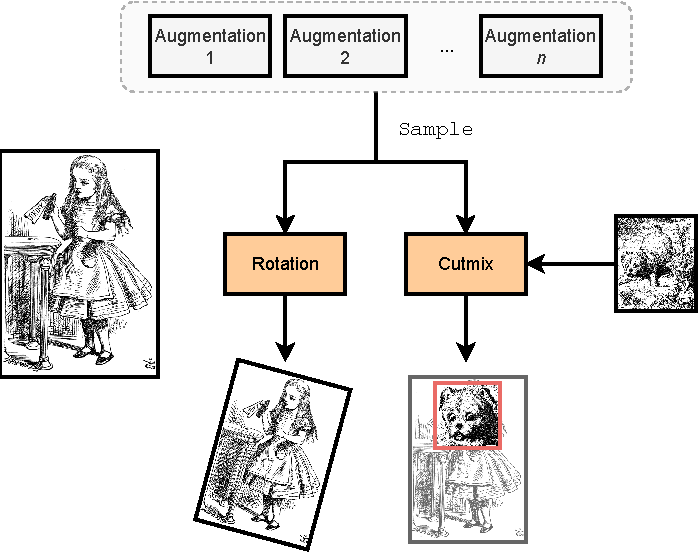
\includegraphics[width=0.7\textwidth]{images/data_augmentation}
    \caption{Общий обзор аугментации данных. Для каждого мини-пакета случайным образом выбирается набор аугментаций данных из базового набора, и они применяются к изображениям мини-пакета. Здесь мы показываем пример \textit{вращения} и пример \textit{cutmix}. Иллюстрации Джона Тенниела, воспроизведены из Wikimedia.}
    \label{fig:cutmix}
\end{figure}

\section{Dropout и нормализация}

Стратегии, которые мы описали в предыдущем разделе, очень общие, в том смысле, что они подразумевают модификации алгоритма оптимизации или самого набора данных, и их можно применять к широкому кругу алгоритмов. 

Вместо этого мы теперь сосредоточимся на трех идеях, которые были популяризированы в период с 2012 по 2016 год, в основном в контексте соревнования ImageNet. Все три специфичны для дифференцируемых моделей, поскольку их можно реализовать как дополнительные слои или соединения в модели, которые упрощают обучение очень глубоких моделей. Мы перечисляем методы примерно в хронологическом порядке. Как мы увидим в оставшихся разделах, эти методы остаются фундаментальными и за пределами свёрточных моделей.

\subsection{Регуляризация с помощью dropout}
\label{subsec:dropout}

При обсуждении аугментации данных мы упоминали, что одна из идей заключается в том, что аугментация заставляет сеть учиться в более сложной обстановке, так что ее производительность в более простой среде может улучшиться с точки зрения точности и устойчивости. \textbf{Dropout} \cite{srivastava2014dropout} расширяет эту идею на внутренние вложения модели: искусственно вводя шум во время обучения в промежуточные выходы модели, решение может улучшиться.

Существует много вариантов возможных типов шума: например, обучение с небольшим количеством гауссовского шума в активации всегда было популярной альтернативой в литературе по рекуррентным моделям. Как следует из названия, идея dropout заключается в случайном удалении определенных блоков (нейронов) во время вычисления, что снижает зависимость от любого отдельного внутреннего признака и (надеюсь) приводит к обучению устойчивых слоев с хорошим количеством избыточности.

\begin{figure}
    \centering
    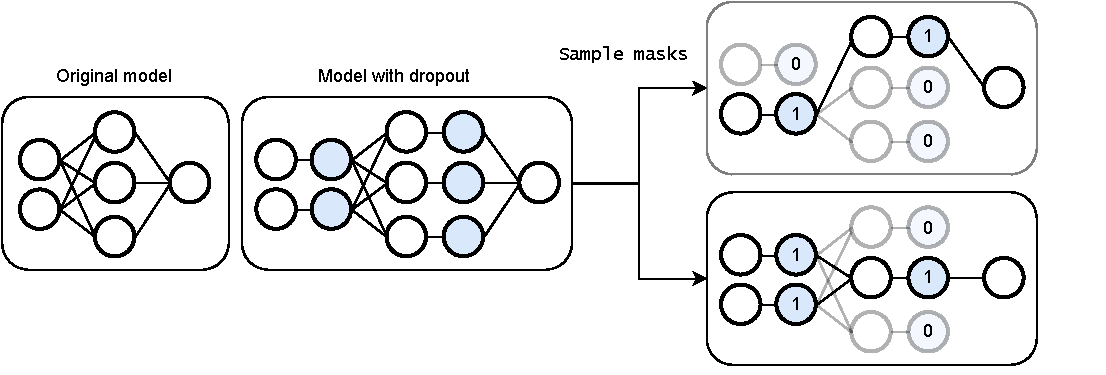
\includegraphics[width=0.95\textwidth]{images/dropout}
    \caption{Схематический обзор dropout: начиная с базовой модели, мы добавляем дополнительные блоки после каждого интересующего слоя, показанные синим цветом. Во время обучения каждому блоку dropout случайным образом присваивается двоичное значение, маскируя часть предыдущих слоев. Следовательно, мы выбираем одну из экспоненциально многих возможных моделей, имеющих подмножество активных скрытых блоков, каждый раз, когда выполняется прямой проход. Dropout также можно применять на уровне входа, случайным образом удаляя некоторые входные признаки.}
    \label{fig:dropout}
\end{figure}

Мы определяем dropout в случае полносвязного слоя, что является его наиболее распространенным применением. 

\begin{definition}[Слой Dropout] \addbottle
\%
Обозначим через $\mathbf{X} \sim (n, c)$ мини-пакет внутренних активаций модели (например, выход некоторого промежуточного полносвязного слоя) с $n$ элементами в мини-пакете и $c$ признаками. В слое dropout мы сначала выбираем бинарную матрицу $\mathbf{M} \sim \text{Binary}(n,c)$ того же размера, элементы которой взяты из распределения Бернулли с вероятностью $p$ (где $p \in [0,1]$ — гиперпараметр пользователя):\footnote{Выборки из $\text{Bern}(p)$ равны $1$ с вероятностью $p$ и $0$ с вероятностью $1-p$.}
\%
\begin{equation}
M_{ij}\sim \text{Bern}(p)
\label{eq:sampling_m}
\end{equation}
\%
Выход слоя получается путем маскирования входа:
\%
$$
\textnormal{Dropout}(\mathbf{X})=\mathbf{M} \odot \mathbf{X}
$$
\%
Слой имеет один гиперпараметр, $p$, и не имеет обучаемых параметров.
\%
\end{definition}
\%
Мы называем $1-p$ \textbf{вероятностью отсева}. Следовательно, для любого элемента в мини-пакете случайное количество блоков (примерно $(1-p) \%$) будет установлено в ноль, эффективно удаляя их. Это показано на Рисунке \ref{fig:dropout}, где дополнительные блоки dropout показаны синим цветом. Выборка маски является частью прямого прохода слоя: для двух разных прямых проходов выход будет разным, поскольку будут замаскированы разные элементы, как показано справа на Рисунке \ref{fig:dropout}. 

Как показывает рисунок, мы можем реализовать dropout как слой, который вставляется после каждого слоя, который мы хотим отсеять. Например, рассмотрим полносвязную модель с двумя слоями, показанную на Рисунке \ref{fig:dropout}:
\%
$$
y=(\text{FC}\circ\text{FC})(\mathbf{x})
$$
\%
Добавление регуляризации dropout к входу и к выходу первого слоя возвращает новую модель, имеющую \textit{четыре} слоя:
\%
$$
y=(\text{FC}\circ{\color{drawred}\text{Dropout}}\circ\text{FC} \circ {\color{drawred}\text{Dropout}})(\mathbf{x})
$$
\%
См. Листинг \ref{code:dropout_model} для реализации в PyTorch.

\begin{mypy}{Модель на Рисунке \ref{fig:dropout}, реализованная как последовательность из четырех слоев в PyTorch. Во время обучения выход модели будет стохастическим из-за наличия двух слоев dropout.}{code:dropout_model}
model = nn.Sequential(
    nn.Dropout(0.3),
    nn.Linear(2, 3), nn.ReLU(),
    nn.Dropout(0.3),
    nn.Linear(3, 1)
)
\end{mypy}

Хотя dropout может улучшить производительность, выход $y$ теперь является случайной величиной по отношению к выборке различных масок внутри слоев dropout, что нежелательно после обучения. Например, два прямых прохода сети могут вернуть два разных выхода, и некоторые выборки (например, с очень большим количеством нулей) могут быть неоптимальными. Следовательно, нам нужна некоторая стратегия для замены прямого прохода детерминированной операцией. 

Предположим, у нас есть $m$ слоев dropout. Обозначим через $\mathbf{M}_i$ маску в $i$-м слое dropout, через $p(\mathbf{M}_1, \ldots, \mathbf{M}_m) = \prod_{i=1}^m p(\mathbf{M}_i)$ — распределение вероятностей по объединению масок, а через $f(\mathbf{x}; \mathbf{M})$ — детерминированный выход после выбора заданного набора масок $\mathbf{M} \sim p(\mathbf{M})$. Один из вариантов — заменить эффект dropout его математическим ожиданием во время вывода:
\%
$$
f(\mathbf{x})=\begin{cases} f(\mathbf{x}; \mathbf{M}), \;\; \mathbf{M}\sim p(\mathbf{M}) & \texttt{ [обучение]} \\ \mathbb{E}_{p(\mathbf{M})}\left[f(\mathbf{x}; \mathbf{M})\right]  & \texttt{ [вывод]}\end{cases}
$$
\%
Мы можем аппроксимировать математическое ожидание с помощью выборки Монте-Карло (Приложение \ref{chap:probability_theory}), многократно выбирая значения масок и усредняя:
\%
$$
\mathbf{E}_{p(\mathbf{M})}\left[f(\mathbf{x}; \mathbf{M})\right] \approx \frac{1}{k}\sum_{i=1}^k f(\mathbf{x}; \mathbf{Z}_i),\;\; \mathbf{Z}_i \sim p(\mathbf{M})
$$
\%
что является просто средним от $k$ прямых проходов. Это называется \textbf{dropout Монте-Карло} \cite{gal2016dropout}. Выход по-прежнему стохастический, но при правильном выборе $k$ дисперсию можно сдержать. Кроме того, выходы разных прямых проходов могут дать меру неопределенности предсказания. 

Однако выполнение нескольких прямых проходов может быть дорогостоящим. Более простой (и более распространенный) вариант — заменять случайные величины \textit{послойно}, что является разумным приближением. Математическое ожидание в этом случае можно записать в замкнутой форме:
\%
$$
\mathbb{E}_{p(\mathbf{M})}\left[\text{Dropout}(\mathbf{X})\right]=p\mathbf{X}
$$
\%
что является входом, масштабированным на постоянный коэффициент $p$ (вероятность выбора $1$ в маске). Это приводит к еще более простой формулировке, \textbf{инвертированному dropout}, где эта поправка учитывается во время обучения:
\%
$$
\text{Dropout}(\mathbf{X})=\begin{cases} \displaystyle\frac{\mathbf{M}\odot\mathbf{X}}{(1-p)} & \texttt{ [обучение]} \\ \;\;\mathbf{X}  & \texttt{ [вывод]}\end{cases}
$$
\%
В этом случае слой dropout не имеет эффекта при применении во время вывода и может быть напрямую удален. Это предпочтительная реализация в большинстве фреймворков. См. Листинг \ref{code:dropout} для некоторых сравнений.

\begin{mypy}{Применение модели из Листинга \ref{code:dropout_model} к мини-пакету из $16$ примеров. Для слоев, таких как dropout, фреймворку требуется способ различать прямой проход, выполняемый во время обучения или во время вывода. В PyTorch это делается путем вызова методов {\footnotesize\mintinline{python}{train}} и {\footnotesize\mintinline{python}{eval}} модели, которые устанавливают внутренний флаг {\footnotesize\mintinline{python}{train}} для всех слоев. Мы также показываем векторизованную реализацию dropout Монте-Карло.}{code:dropout}
x = torch.randn((16, 2))

# Обучение с dropout
model.train()
y = model(x)

# Вывод с dropout
model.eval()
y = model(x)

# Dropout Монте-Карло для вывода
k = 10
model.train()
y = model(x[:, None, :].repeat(1, k, 1)).mean(1)
\end{mypy}

Как мы уже упоминали, dropout (возможно, с низкой вероятностью отсева, такой как $p=0.1$ или $p=0.2$) распространен для полносвязных слоев. Он также распространен для карт внимания (представленных в следующей главе). Он менее распространен для свёрточных слоев, где отсев отдельных элементов входного тензора приводит к слишком неструктурированным паттернам разреженности. Были разработаны варианты dropout, которые учитывают специфическую структуру изображений: например, \textbf{пространственный dropout} \cite{tompson2015efficient} отсеивает целые каналы тензора, в то время как \textbf{cutout} \cite{devries2017improved} отсеивает пространственные патчи одного канала.

Возможны и другие альтернативы. Например, \textbf{DropConnect} \cite{wan2013regularization} отсеивает отдельные веса полносвязного слоя:
\%
$$
\text{DropConnect}(\mathbf{x})=(\mathbf{M}\odot\mathbf{W})\mathbf{x}+\mathbf{b}
$$
\%
DropConnect при выводе также можно эффективно аппроксимировать с помощью согласования моментов \cite{wan2013regularization}. Однако они менее распространены на практике, и предпочтение отдается техникам, описанным далее.

\subsection{Пакетная (и послойная) нормализация} \addclock

При работе с табличными данными распространенной операцией предварительной обработки, которую мы еще не обсуждали, является \textbf{нормализация}, т.е. обеспечение того, чтобы все признаки (все столбцы входной матрицы) имели схожие диапазоны и статистики. Например, мы можем предварительно обработать данные, чтобы сжать все столбцы в диапазон $[0,1]$ (\textbf{нормализация мин-макс}) или обеспечить нулевое среднее и единичную дисперсию для каждого столбца (называется либо \textbf{стандартным масштабированием}, либо \textbf{нормальным масштабированием}, либо \textbf{масштабированием z-оценки}).

\textbf{Пакетная нормализация} (BN, \cite{ioffe2015batch}) воспроизводит эти идеи, но для промежуточных вложений модели. Это нетривиально, поскольку статистики блока (например, его среднее) будут меняться от итерации к итерации после каждого обновления градиентного спуска. Следовательно, для вычисления среднего значения блока мы должны выполнять прямой проход по всему обучающему набору данных на каждой итерации, что нецелесообразно. Как следует из названия, основная идея BN заключается в аппроксимации этих статистик с использованием только данных \textit{в самом мини-пакете}. 

Снова рассмотрим выход любого полносвязного слоя $\mathbf{X} \sim (n,c)$, где $n$ — размер мини-пакета. Вскоре мы увидим, как расширить эти идеи на изображения и другие типы данных. В BN мы нормализуем каждый признак (каждый столбец $\mathbf{X}$), чтобы он имел нулевое среднее и единичную дисперсию, основываясь только на мини-пакете. Для этого мы начинаем с вычисления эмпирического среднего по столбцам $\mathbf{\mu} \sim (c)$ и дисперсий $\sigma^2 \sim (c)$:
\%
\begin{align}
\text{Среднее столбца } j \text{:}  &&& \mu_j = \frac{1}{n}\sum_iX_{ij} \label{eq:empirical_mean} \\ \text{Дисперсия столбца } j \text{:} &&& \sigma^2_j=\frac{1}{n}\sum_i(X_{ij}-\mu_j)^2  \label{eq:empirical_variance}
\end{align}
\%
Затем мы приступаем к нормализации столбцов:

\vspace{1em}
$$
\mathbf{X}^\prime=\frac{\eqnmarkbox[drawred]{node}{\mathbf{X} - \mu}}{\eqnmarkbox[drawgreen]{node2}{\sqrt{\sigma^2 + \varepsilon}}}
$$
\annotate[yshift=1em]{above,right}{node}{Установить среднее каждого столбца в $0$}
\annotate[yshift=-1em]{below,right}{node2}{Установить дисперсию каждого столбца в $1$}

\vspace{1em}
где мы рассматриваем стандартные правила трансляции ($\mu$ и $\sigma^2$ транслируются по первому измерению), а $\varepsilon > 0$ — это небольшой положительный член, добавленный для предотвращения деления на ноль. В отличие от нормализации для табличных данных, где эта операция применяется один раз ко всему набору данных перед обучением, в BN эта операция должна пересчитываться для каждого мини-пакета во время каждого прямого прохода.

Выбор нулевого среднего и единичной дисперсии — это всего лишь соглашение, не обязательно лучшее. Чтобы обобщить его, мы можем позволить алгоритму оптимизации выбрать лучший вариант за небольшую плату в виде параметров. Рассмотрим два обучаемых параметра $\mathbf{\alpha} \sim (c)$ и $\mathbf{\beta} \sim (c)$ (которые мы можем инициализировать как $1$ и $0$ соответственно), мы выполняем:
\%
$$
\mathbf{X}^{\prime\prime}=\alpha\mathbf{X}^\prime + \beta
$$
\%
с аналогичными правилами трансляции, как и выше. Результирующая матрица будет иметь среднее $\beta_i$ и дисперсию $\alpha_i$ для $i$-го столбца. Слой BN определяется комбинацией этих двух операций.

\begin{definition}[Слой пакетной нормализации] \addbottle
\%
Для входной матрицы $\mathbf{X} \sim (n,c)$ слой \textbf{пакетной нормализации} (BN) применяет следующую нормализацию:
\%
$$
\textnormal{BN}(\mathbf{X})=\alpha\left(\frac{\mathbf{X} - \mu}{\sqrt{\sigma^2 + \varepsilon}}\right) + \beta
$$
\%
где $\mu$ и $\sigma^2$ вычисляются в соответствии с \eqref{eq:empirical_mean} и \eqref{eq:empirical_variance}, а $\alpha \sim (c)$ и $\beta \sim (c)$ являются обучаемыми параметрами. Слой не имеет гиперпараметров. Во время вывода $\mu$ и $\sigma^2$ фиксируются, как описано далее.
\%
\end{definition}
\%
Слой имеет всего $2c$ обучаемых параметров, и можно показать, что он значительно упрощает обучение сложных моделей при вставке между каждым блоком. В частности, обычно рассматривают BN, размещенный между линейными и нелинейными компонентами модели:
\%
$$
\mathbf{H} = (\text{ReLU}\circ {\color{drawred}\text{BN}} \circ \text{Linear})(\mathbf{X})
$$
\%
Центрирование данных перед ReLU может привести к лучшему использованию его отрицательного (разреженного) квадранта. Кроме того, эта схема делает смещение в линейном слое избыточным (поскольку оно сливается с параметром $\beta$), что позволяет его удалить. Наконец, двойная линейная операция может быть легко оптимизирована стандартными компиляторами в большинстве фреймворков.

BN настолько эффективна, что это привело к обширной литературе о понимании причин \cite{bjorck2018understanding}. Первоначальный вывод рассматривал проблему, известную как \textbf{внутренний сдвиг ковариат}, т.е. тот факт, что с точки зрения одного слоя статистики получаемых им входов будут меняться во время оптимизации из-за изменений весов предыдущих слоев. Однако современная литература согласна с тем, что эффекты BN более очевидны в самой оптимизации, как с точки зрения стабильности, так и с точки зрения возможности использования более высоких скоростей обучения, из-за комбинации эффектов масштабирования и центрирования на градиентах \cite{bjorck2018understanding}.\footnote{См. также \url{https://iclr-blog-track.github.io/2022/03/25/unnormalized-resnets/} для хорошей отправной точки в эту литературу (и соответствующую литературу по разработке \textbf{моделей без нормализаторов}.}

Расширение BN за пределы табличных данных просто. Например, рассмотрим мини-пакет вложений изображений $X \sim (n,h,w,c)$. Мы можем применить BN к каждому каналу, рассматривая первые три измерения вместе, т.е. мы вычисляем среднее по каналам как:

$$
\mu_z = \eqnmarkbox[drawred]{node}{\frac{1}{nhw}\sum_{i, j,k} X_{ijkz}}
$$
\annotate[yshift=-1em]{below,right
}{node}{Среднее канала $z$ (все пиксели, все изображения)}

\vspace{0.5em}
\subsubsection*{Пакетная нормализация во время вывода}

BN вводит зависимость между предсказанием для входа и мини-пакетом, в котором он находится, что нежелательно во время вывода (иначе говоря, перемещение изображения из одного мини-пакета в другой изменит его предсказание). Однако мы можем использовать тот факт, что параметры модели не меняются после обучения, и мы можем заморозить среднее и дисперсию на заданном значении. Для этого есть две возможности:
\%
\begin{enumerate}
\item После обучения мы выполняем еще один прямой проход по всему обучающему набору, чтобы вычислить эмпирическое среднее и дисперсию по отношению к набору данных \cite{wu2021rethinking}.
\item Чаще мы можем поддерживать скользящий набор статистик, которые обновляются после каждого прямого прохода модели во время обучения, и использовать их после обучения. Рассматривая только среднее для простоты, предположим, мы инициализируем другой вектор $\widehat{\mu} = \mathbf{0}$, соответствующий «скользящему среднему среднего». После вычисления $\mu$ как в \eqref{eq:empirical_mean}, мы обновляем скользящее среднее с помощью экспоненциального скользящего среднего:
    \%
    $$
    \widehat{\mu} \gets \lambda\widehat{\mu} + (1-\lambda)\mu
    $$
    где $\lambda$ установлено на небольшое значение, например, $\lambda=0.01$. Предполагая, что обучение сходится, скользящее среднее также сойдется к аппроксимации среднего, заданной вариантом (1).\footnote{$\widehat{\mu}$ — это первый пример тензора слоя, который является частью состояния слоя, адаптируется во время обучения, но не нужен для градиентного спуска. В PyTorch они называются \textit{буферами}.}
\end{enumerate}    

\subsubsection*{Варианты пакетной нормализации}

Несмотря на свою хорошую эмпирическую производительность, у BN есть несколько важных недостатков. Мы уже упоминали зависимость от мини-пакета, которая имеет и другие последствия: например, дисперсия $\mu$ во время обучения будет расти для небольших мини-пакетов, и обучение может быть невозможным для очень малых размеров мини-пакетов. Кроме того, обучение может быть затруднено в распределенных контекстах (где каждый GPU содержит отдельную часть мини-пакета). Наконец, замена $\mu$ на другое значение после обучения создает нежелательное несоответствие между обучением и выводом.

Были предложены варианты BN для решения этих проблем. Распространенная идея — сохранить общую структуру слоя, но изменить оси, по которым выполняется нормализация. Например, \textbf{послойная нормализация} \cite{ba2016layer} вычисляет эмпирическое среднее и дисперсию по \textit{строкам} матрицы, т.е. для каждого входа независимо:

\begin{align}
\text{Среднее {\color{drawred}строки} $i$:} &&& \mu_i = \frac{1}{\color{drawred}c}\sum_jX_{\color{drawred}ji}  \\ 
\text{Дисперсия {\color{drawred}строки} $i$:}  &&& \sigma^2_i=\frac{1}{\color{drawred}c}\sum_j(X_{\color{drawred}ji}-\mu_i)^2  
\end{align}

\begin{SCfigure}
    \centering
    \hspace{0.5em}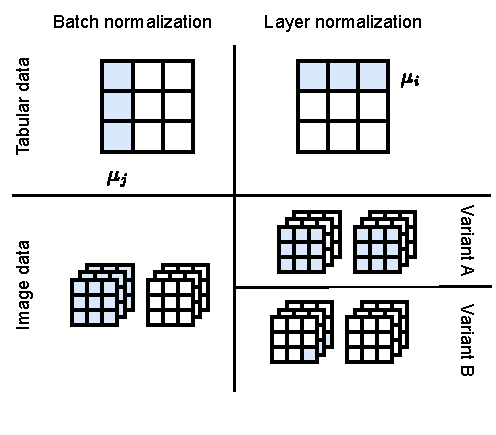
\includegraphics[width=0.6\textwidth]{images/layer_normalization}
    \caption{Сравнение между BN и LN для табличных и изображенческих данных. Синие области показывают наборы, по которым мы вычисляем средние и дисперсии. Для LN у нас есть два варианта, обсуждаемых подробнее в основном тексте.}
    \label{fig:layer_normalization}
\end{SCfigure}

Рассмотрим Рисунок \ref{fig:layer_normalization}, где мы показываем сравнение между BN и LN для табличных и изображенческих данных. В частности, мы показываем синим цветом все сэмплы, используемые для вычисления одного среднего и дисперсии. Для послойной нормализации мы можем вычислять статистики по $h,w,c$ одновременно (вариант А) или для каждого пространственного местоположения отдельно (вариант Б). Последний выбор распространен в моделях-трансформерах, обсуждаемых в следующей главе. Возможны и другие варианты, например, \textbf{групповая нормализация} ограничивает операцию подмножеством каналов, причем случай одного канала известен как \textbf{инстанс-нормализация}.\footnote{См. \url{https://iclr-blog-track.github.io/2022/03/25/unnormalized-resnets/} для более красивого варианта Рисунка \ref{fig:layer_normalization}.}

В BN оси, по которым мы вычисляем статистики в \eqref{eq:empirical_mean} и \eqref{eq:empirical_variance}, совпадают с осями, по которым мы применяем обучаемые параметры. В LN эти два аспекта разделены. Например, рассмотрим слой LN в PyTorch, применяемый к мини-пакетам размерности $(b, 3, 32, 32)$:

{\footnotesize
\noindent\mintinline{python}{ln = nn.LayerNorm(normalized_shape=[3, 32, 32])}
}

Это соответствует варианту А на Рисунке \ref{fig:layer_normalization}. В этом случае $\alpha$ и $\beta$ будут иметь ту же форму, что и оси, по которым мы вычисляем нормализацию, т.е. $\alpha, \beta \sim (3,32,32)$, всего $2\times3\times32\times32=6144$ обучаемых параметров. Конкретная реализация LN и BN должна проверяться для каждого фреймворка и модели.

В заключение мы упомянем еще один распространенный вариант послойной нормализации, называемый нормализацией \textbf{среднеквадратичного корня} (RMSNorm) \cite{zhang2019root}. Он упрощает LN, удаляя центрирование и сдвиг среднего, что для одного входного вектора $\mathbf{x} \sim (c)$ можно записать как:
\%
\begin{equation}
\text{RMSNorm}(\mathbf{x}) = \frac{\mathbf{x}}{\sqrt{\frac{1}{c}\sum_i x_i^2}} \odot \mathbf{\alpha} 
\end{equation}
\%
Когда $\mathbf{\beta} = 0$ и данные уже центрированы по нулю, LN и RMSNorm идентичны.

\section{Остаточные соединения}
\label{sec:residual_connections}
\subsection{Остаточные соединения и остаточные сети} \addclock

Комбинация всех техник, рассмотренных в предыдущем разделе, достаточна для значительного увеличения числа слоев в наших моделях, но только до определенного верхнего предела. Рассмотрим три общие последовательности слоев $f_1$, $f_2$ и $f_3$, и две модели, где одна является подмножеством другой:
\%
\begin{gather*}
g_1(x) = (f_3 \circ f_1)(x) \\ g_2(x)=(f_3\circ {\color{drawred}f_2}\circ f_1)(x)
\end{gather*}
\%
Интуитивно, по теореме об универсальной аппроксимации всегда должно быть возможно, чтобы промежуточная часть, $f_2$, аппроксимировала тождественную функцию $f_2(x) \approx x$, и в этом случае $g_2(x) \approx g_1(x)$. Следовательно, всегда существует такая настройка параметров, при которой вторая (более глубокая) модель должна работать по крайней мере так же хорошо, как и первая (более мелкая). Однако на практике этого не наблюдалось, как показано на Рисунке \ref{fig:resnet}.

\begin{SCfigure}
    \centering
    \hspace{1em}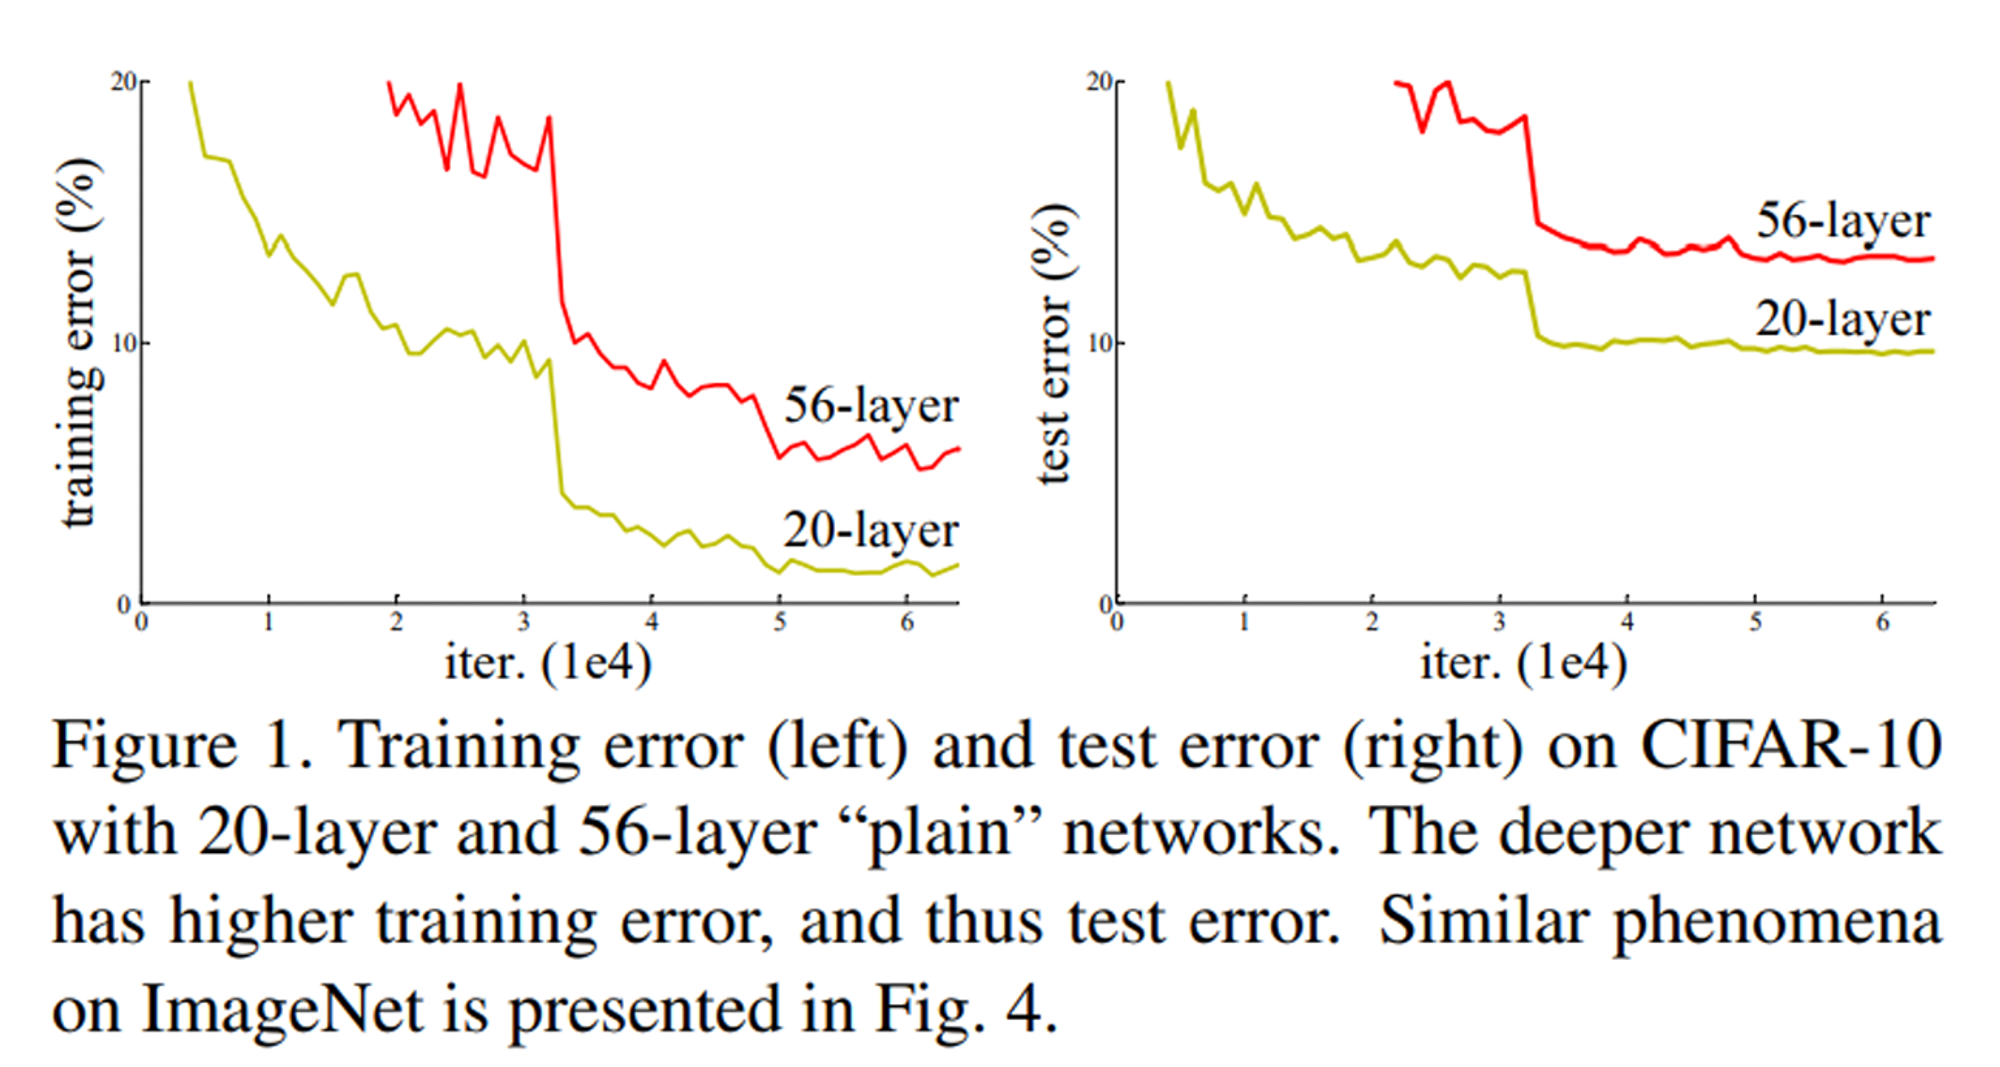
\includegraphics[width=0.6\textwidth]{images/resnet}
    \caption{Более крупные модели не всегда монотонно улучшают ошибку обучения, несмотря на то, что представляют более крупные классы функций. Воспроизведено из \cite{he2016deep}.}
    \label{fig:resnet}
\end{SCfigure}

Мы можем решить эту проблему, смещая блоки в сети к тождественной функции. Это можно легко сделать, переписав блок $f(x)$ с помощью так называемого \textbf{остаточного (пропускающего) соединения} \cite{he2016deep}:
\%
$$
r(x)=f(x){\color{drawred} \; + \;x}
$$
\%
Следовательно, мы используем блок для моделирования отклонений от тождества, $f(x) = r(x) - x$, вместо моделирования отклонений от нулевой функции. Этот небольшой трюк сам по себе помогает в обучении моделей до сотен слоев. Мы называем $f(x)$ \textbf{остаточным путем}, $r(x)$ — \textbf{остаточным блоком}, а свёрточную модель, состоящую из остаточных блоков, — \textbf{остаточной сетью} (сокращенно ResNet).

Остаточные соединения хорошо работают с пакетной нормализацией на остаточном пути, что, как можно показать, дополнительно смещает модель к тождеству в начале обучения \cite{de2020batch}. Однако остаточные соединения можно добавлять только в том случае, если размерность входа и выхода $f(x)$ идентична. В противном случае к остаточному соединению можно добавить некоторое перемасштабирование. Например, если $x$ — это изображение, а $f(x)$ изменяет количество каналов, мы можем добавить свёртку $1 \times 1$:
\%
$$
r(x)=f(x)+\text{Conv2D}_{1\times 1}(x)
$$
\%
Преимущество остаточного блока можно понять также с точки зрения его обратного прохода. Рассмотрим VJP остаточного блока:
\%
$$
\text{vjp}_r(\mathbf{v})=\text{vjp}_f(\mathbf{v}) + \mathbf{v}^\top\mathbf{I} = \eqnmarkbox[drawred]{node}{\text{vjp}_f(\mathbf{v})} + \eqnmarkbox[drawgreen]{node2}{\mathbf{v}^\top}
$$
\annotate[yshift=-1em]{below,left}{node}{VJP $f$}
\annotate[yshift=-3em]{below,left}{node2}{VJP пропускающего соединения}

\vspace{2em}
Следовательно, прямой проход пропускает вход $x$ без изменений по пропускающему соединению, в то время как обратный проход добавляет неизмененный обратно распространенный градиент $\mathbf{v}$ к исходному VJP, что может помочь смягчить нестабильность градиента.

\subsection*{О проектировании остаточного блока}

Как спроектировать блок $f(x)$? Рассмотрим пакетно-нормализованный блок, представленный ранее:
\%
$$
h = \underbrace{(\text{ReLU}\circ \text{BN} \circ \text{Conv2D})}_{=f(x)}(x) + x
$$
\%
Поскольку выход ReLU всегда положителен, мы имеем, что $h \ge x$ (поэлементно). Следовательно, стек остаточных блоков такой формы может только увеличивать значения входного тензора или устанавливать его в ноль. По этой причине исходный дизайн, предложенный в \cite{he2016deep}, рассматривал стек блоков такой формы, удаляя последнюю функцию активации. В качестве примера, для двух блоков мы получаем следующий дизайн:
\%
$$
h = (\text{BN} \circ \text{Conv2D} \circ\text{ReLU}\circ \text{BN} \circ \text{Conv2D})(x) + x
$$
\%
Серии блоков такой формы может предшествовать небольшой компонент с неостаточными соединениями для уменьшения размерности изображения, иногда называемый \textbf{стволом}. Конкретный выбор гиперпараметров для этого блока значительно менялся с годами.

\begin{SCfigure}
    \centering
    \hspace{1em}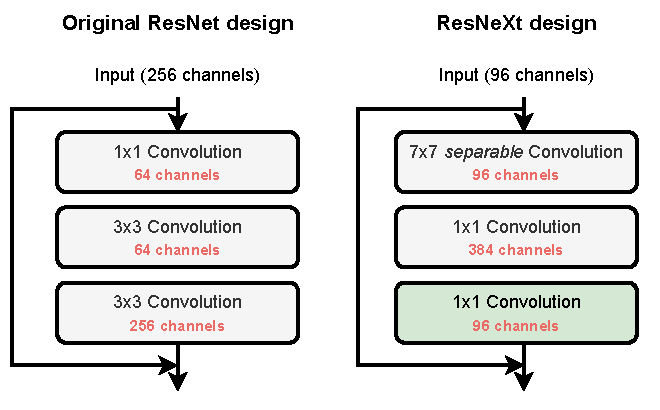
\includegraphics[width=0.6\textwidth]{images/resnet_design}
    \caption{Исходный блок ResNet \cite{he2016deep} и более поздний блок ResNeXt \cite{liu2022convnet}. Как видно, дизайн сместился от раннего уменьшения каналов к более позднему сжатию (\textbf{бутылочное горлышко}). Дополнительные детали (не показаны) — это переход от BN к LN и использование функций активации GELU. Адаптировано из \cite{liu2022convnet}.}
    \label{fig:resnext}
\end{SCfigure}

Исходный блок ResNet предлагал сжатие количества каналов для первой операции, за которым следовала стандартная свёртка $3 \times 3$ и окончательное увеличение количества каналов. В последнее время, напротив, стали популярны слои \textbf{бутылочного горлышка}, такие как блок v \cite{liu2022convnet} (справа на Рисунке \ref{fig:resnext}). Чтобы увеличить рецептивное поле свёртки, начальный слой заменяется глубинной свёрткой. Чтобы использовать уменьшенное количество параметров, количество каналов \textit{увеличивается} на заданный коэффициент (например, в $3\times$, $4\times$), а затем уменьшается последней свёрткой $1\times1$.

\subsection{Дополнительные перспективы остаточных соединений} \addteacup

Мы завершаем главу, обсуждая две интересные перспективы использования остаточных соединений, которые обе были подробно исследованы в текущих исследованиях. Во-первых, рассмотрим сеть, состоящую из двух остаточных блоков:
\%
\begin{gather}
h_1 = {\color{drawred}f_1}(x)+x\\h_2={\color{drawgreen}f_2}(h_1)+h_1
\end{gather}
\%
Если мы развернем вычисление:
\%
$$
h_2 = {\color{drawgreen}f_2}({\color{drawred}f_1}(x) + x) + {\color{drawred}f_1}(x) + x
$$
\%
Это соответствует сумме нескольких \textit{путей} в сети, где вход либо остается неизменным, либо проходит только через одно преобразование ($f_1$ или $f_2$), либо через их комбинацию.

\begin{SCfigure}
    \centering
    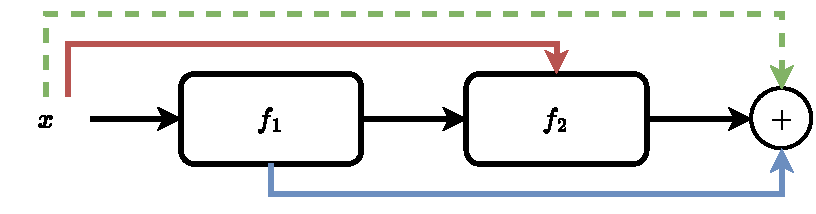
\includegraphics[width=0.6\textwidth]{images/residual_paths}
    \caption{Остаточные пути: черный, красный и синий пути реализованы явно; зеленый путь является только неявным.}
    \label{fig:residual_paths}
\end{SCfigure}

Должно быть ясно, что количество таких путей растет экспоненциально с числом остаточных блоков. Следовательно, глубокие остаточные модели можно рассматривать как комбинацию (ансамбль) очень большого числа меньших моделей, реализованных через разделение весов. Эту точку зрения можно проверить, чтобы показать, например, что ResNet, как правило, устойчивы к небольшим удалениям или модификациям своих элементов \cite{veit2016residual}. Это визуально показано на Рисунке \ref{fig:residual_paths}.

Во-вторых, рассмотрим следующее дифференциальное уравнение, выраженное в терминах непрерывного параметра $t$, представляющего время:
\%
$$
\partial_tx_t=f(x,t)
$$
\%
Мы используем нейронную сеть с аргументами $x$ и $t$ (скаляр) для параметризации производной по времени некоторой функции. Это называется \textbf{обыкновенным дифференциальным уравнением} (ОДУ). Распространенной проблемой с ОДУ является интегрирование от известного начального значения $x_0$ до некоторого заданного момента времени $T$:
\%
$$
x_T=x_0+\int_{t=0}^Tf(x,t)dt
$$
\%
Метод Эйлера\footnote{\url{https://en.wikipedia.org/wiki/Euler_method}} для вычисления $x_T$ работает путем выбора небольшого шага $h$ и итеративного вычисления дискретизации первого порядка:
\%
$$
x_t=x_{t-1}+hf(x_{t-1}, t)
$$
\%
Объединяя $h$ в $f$, это соответствует ограниченной форме остаточной модели, где все остаточные блоки разделяют одни и те же веса, каждый слой соответствует дискретизированному моменту времени, а $x_T$ — это выход сети. С этой точки зрения мы можем напрямую работать с исходным уравнением в непрерывном времени и вычислять выход, интегрируя его с помощью современных решателей ОДУ. Это называется \textbf{нейронным ОДУ} \cite{chen2018neural}. Можно вывести варианты обратного распространения ошибки в непрерывном времени, которые принимают форму другой задачи ОДУ. В следующем томе мы увидим интересную связь между нейронными ОДУ и классом генеративных моделей, известных как \textbf{нормализующие потоки} \cite{papamakarios2021normalizing}.

\section*{От теории к практике}

\begin{wrapfigure}{r}{3.0cm}
\vspace{-3em}
\includegraphics[width=3.0cm]{images/shutterstock_2075221579.jpg}
\vspace{-2em}
\end{wrapfigure}

Все слои, которые мы обсуждали в этой главе (пакетная нормализация, dropout, ...), уже реализованы в PyTorch, Equinox и практически в любом другом фреймворке. Что касается остальных описанных нами техник, это зависит от фреймворка: например, затухание весов реализовано нативно во всех оптимизаторах PyTorch, аугментацию данных можно найти как преобразования внутри \texttt{torchvision} (и других соответствующих библиотек), в то время как раннюю остановку необходимо реализовывать вручную.\footnote{В PyTorch распространенной альтернативой является использование внешней библиотеки, такой как PyTorch Lightning, для управления процессом обучения. Модификации процедуры обучения, такие как ранняя остановка, предварительно реализованы в виде функций \textit{обратного вызова}.}

\begin{enumerate}
\item Прежде чем переходить к следующей главе, я предлагаю вам попробовать реализовать либо dropout, либо пакетную нормализацию как слой, используя только стандартные процедуры линейной алгебры, сравнивая результаты со встроенными слоями.
\item В Главе \ref{chap:cnns} вы должны были реализовать простую свёрточную модель для классификации изображений. Попробуйте постепенно увеличивать ее размер, добавляя по мере необходимости нормализацию, dropout или остаточные соединения.
\item Возьмите стандартную архитектуру, такую как ResNet \cite{he2016deep} или ResNeXt \cite{liu2022convnet}. Попробуйте реализовать всю модель, следуя предложениям из оригинальных статей. Обучение на наборах данных, подобных ImageNet, может быть сложным на потребительских GPU — если у вас нет доступа к хорошему оборудованию или часам облачных GPU, вы можете продолжать сосредотачиваться на более простых наборах данных, таких как CIFAR-10.
\item К этому моменту вы, возможно, поняли, что обучение с нуля очень больших моделей (например, ResNet-50) на небольших наборах данных практически невозможно. Одним из решений является инициализация весов модели из онлайн-репозитория, используя, например, веса модели, обученной на ImageNet, и \textbf{дообучение} модели путем изменения последнего слоя, соответствующего классификационной голове. К этому моменту книги это должно показаться относительно простым — я предлагаю использовать одну из многих предварительно обученных моделей, доступных на torchvision или на Hugging Face Hub.\footnote{Для примера руководства: \url{https://pytorch.org/tutorials/beginner/transfer_learning_tutorial.html}.} Мы рассмотрим дообучение более подробно в следующем томе.

\end{enumerate}